\lohead{Vollmaier Alois}

\chapter{Informatik}

\section{Visualisierte Benutzeroberfläche}
\label{sec:gui}
\subsection{Konzept}

\subsection{Auswahl des GUI-Toolkits}
\subsubsection{Swing}
\subsubsection{JavaFX}
\subsubsection{Qt}

\subsection{Das MVC-Design Pattern}
\subsubsection{Grundlagen}
\subsubsection{Integration des Patterns in die GUI}

\subsection{Auswahl der IDE}

\section{Kommunikation}
\label{sec:communication}
\subsection{Konzept}

Um erfolgreich Daten zwischen dem Raspberry PI 3B+ und der Platine, welche die Ansteuerung sämtlicher Komponenten übernimmt, zu übertragen, wird ein Kommunikationsprotokoll benötigt.
Dieses Protokoll stellt im engsten Sinne eine Vereinbarung dar, wie die Datenübertragung zwischen zwei oder mehreren Parteien abläuft. Anforderungen an dieses Protokoll sollen sein:
\begin{enumerate}
    \item einfache Integration in die Zielsysteme
    \item erweiterbarkeit des Protokolls mit geringem Arbeitsaufwand
    \item hohe Sicherheit gegenüber Übertragungsfehler
    \item schnelle Fehlererkennung sowie Fehlerbehebung
\end{enumerate}
Neben standartisierten Protokollen wie Modbus, Feldbus oder CAN-Bus gibt es die Möglichkeit selbst ein sogenanntes propretäres Übertragungsprotokoll zu kreieren. Dies ist in unserem Fall nötig, um alle Anforderungen abzudecken.
Basierend auf dem Master - Slave Prinzip, wobei der Rasperry PI den Master und die Ansteuerplatine den Slave darstellt, soll ein abgewandeltes Modbus ASCII Protokoll umgesetzt werden.

Zusätzlich soll, um die Anforderung des einfachen Fehlerhandlings zu erfüllen, ein Simulator ausprogrammiert werden, welcher auf Softwarebebene den Platz des Slaves bzw. der Ansteuerplatine einnimmt.
Der Startvorgang des Simulators soll mit einer einfachen modifizierung der Konfigurationsdatei vonstatten gehen.

\begin{figure}[H]
    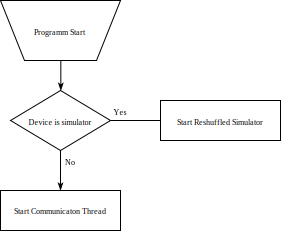
\includegraphics[width=1\textwidth]{fig/ainf/DeviceSelection}
    \caption{Schematische darstellung der Geräteauswahl}
\end{figure}

\subsection{Kommunikation - serielle Schnittstelle}
\subsubsection{Das Übertragungsprotokoll}
\begin{table}[h]
    \centering
    \begin{tabular}{|
    >{\columncolor[HTML]{FFFFFF}}l |
    >{\columncolor[HTML]{FFFFFF}}l |
    >{\columncolor[HTML]{FFFFFF}}l |
    >{\columncolor[HTML]{FFFFFF}}l |
    >{\columncolor[HTML]{FFFFFF}}l |}
        \hline
        \textbf{Doppelpunkt :} & \textbf{Daten (ASCII)} & \textbf{Trennzeichen \#} & \textbf{CRC32-Prüfsumme} & \textbf{Semicolon \textbackslash{}n} \\ \hline
        8-Bit & 16-Bit & 8-Bit & 32-Bit & 8-Bit                                \\ \hline
    \end{tabular}
    \caption{Visualisierung des Datenakets}
\end{table}

Das verbindugslose Protokoll ist wie in der Konzeptbeschreibung Master-Slave orientiert. Die Datenübertragung erfolgt textuell wobei nur Großbuchstaben verwendet werden dürfen.\newline\newline
Wie aus der oben dargestellten Tabelle zu entnehmen, ist der Aufbau eines Frames klar definiert. Der eindeutige Start des Datenpakets, welcher mit einem Doppelpunkt (:) eingeleitet wird, sowie das ebenfalls eindeutige Ende, umgesetzt mit einem Line Feed Character (),
bringt eindeutige Vorteile mit sich. Im Gegensatz zu anderen Protokollen wie z.B. Modbus RTU, muss hier nicht auf das Ende des Pakets "gewartet" werden. Dies führ oft zu Einbußen im Bereich der Performance und ist für uns nicht zielführend.\newline\newline
Gefolgt von dem Startzeichen folgen nun die Daten. Diese beinhalten eindeutig definierte Zecichenfolgen, welche verwendet werden um verschiedenste Zustände der Ansteuerplatine auszuführen. Diese Um auch hier zu wissen, wo sich das der Nutzdaten befindet, schließt das Trennzeichen () diese ab.\newline\newline
Um nun die Integrität, also die Korrektheit der Daten bei einer Übertragung zu überprüfen, wird im nächsten Schritt eine Prüfsumme verwendet. Ziel dieser ist es, anhand der Nutzdaten einen Wert zu bilden, welcher danach vom Sender im Frame gespeichert bzw übertragen wird.
Der Empfänger berechnet nun mit dem selben Verfahren die Prüfsumme aus den empfangenen Daten und vergleicht diese mit der Übertragenen Prüfsumme des Senders. Sind beide Prüfsummen identisch, war die Übertragung erfolgreich und die Daten sind mit großer Wahrscheinlichkeit korrekt.
Stimmen diese nicht überein liegt ein Fehler vor. Die wichtigsten Arten von Übertragungsfehlern sind:
\begin{enumerate}
    \item Einzelbitfehler (1 Bit verändert)
    \item Burstfehler (ganze Folge von Bits verändert)
\end{enumerate}

Neben einfachen Verfahren wie z.B. dem Paritätsbit-Verfahren gibt es auch Komplexere. Die zyklische Redundanzprüfung, auch CRC genannt, ist eines davon. Sie ist realtiv einfach zu realisieren und dennoch wirkungsvoll.
Wichtig beim CRC-Verfahren ist, dass beide Teilnehmen, also Sender und Empfänger, das selbe Generator-Polynom verwenden. Der Grad des Generatorpolyoms beträgt in unserem Fall 32 (CRC-32).



\subsubsection{Die Klasse Serial}
\subsubsection{Die Klasse Communication}
\subsubsection{Die abstrakte Klasse Request und deren abstammende Klassen}
\subsubsection{Die Klasse Response}

\subsection{Kommunikation - Debugging Simulator}

\subsubsection{Die Klasse ReShuffledMainboardSimulator}
\subsubsection{Konzept zum Datenaustausch zwischen Programm und Simulator}

\subsubsection{Die Klassen SimInput- und SimOutputStreamBuffer}
\section{Konfigurationsdatei}
\label{sec:config}
\subsection{Konzept}
\subsection{Umsetzung mithilfe der Klasse Config}
